\documentclass[letterpaper,twocolumn,superscriptaddress,showkeys,longbibliography]{revtex4-1}
\usepackage[utf8]{inputenc}
\usepackage{color,dcolumn,graphicx,hyperref}
\hypersetup
{
    colorlinks = true, linkcolor = blue, citecolor = blue, urlcolor = blue,
}

\begin{document}

\title{Developing a public preprint culture in biology}

\author{Philippe Desjardins-Proulx}
\email[E-mail: ]{philippe.d.proulx@gmail.com}
\affiliation{Theoretical Ecosystem Ecology laboratory, Universit\'e du Qu\'ebec \`a Rimouski, Canada.}
\affiliation{Quebec Center for Biodiversity Science, McGill University, Canada.}

\author{Ethan P. White}
\affiliation{Departement of Bology, Utah State University, United-States of America.}

\author{Joel J. Adamson}
\affiliation{Ecology, Evolution and Organismic Biology, University of North 
Carolina at Chapel Hill, United-States of America}

\author{Timoth\'ee Poisot}
\affiliation{Theoretical Ecosystem Ecology laboratory, Universit\'e du Qu\'ebec \`a Rimouski, Canada.}
\affiliation{Quebec Center for Biodiversity Science, McGill University, Canada.}
\affiliation{International Network for Next-Generation Ecology.}

\author{Karthik Ram}
\affiliation{Environmental Science, Policy, and Management. University of California, Berkeley, United-States of America.}

\author{Dominique Gravel}
\affiliation{Theoretical Ecosystem Ecology laboratory, Universit\'e du Qu\'ebec \`a Rimouski, Canada.}
\affiliation{Quebec Center for Biodiversity Science, McGill University, Canada.}

\keywords{Publishing; Preprint servers; Green Open Access; arXiv.}

\maketitle

\section{Introduction}

%%% TP Oct 11 2012
%%% Just something I am thinking about now
%%% We are not a good sample of biologists. We are mostly evolutionary ecologists,
%%% and perhaps having the input of a "real" (labcoat wearing) biologist can help. 

Public preprint servers allow authors to make manuscripts publicly available
before, or in parallel to, submitting them to journals for traditional
peer-review. The rationale for preprint servers is fundamentally simple: to make
the results of scientific research available to the scientific community as soon
as possible, instead of waiting until the peer-review process is fully
completed.  Sharing manuscripts using preprint servers has numerous advantages
including: 1) rapid dissemination of work-in-progress to a wider audience; 2)
improved peer review by encouraging feedback from the entire research community;
and 3) a fair and straightforward way to establish precedence.

Open preprint servers offer a great opportunity for open science, especially if
the community embraces the idea of discussing preprints. Initiatives like
Haldane's Sieve (\href{http://haldanessieve.org/}{http://haldanessieve.org/}), a
new blog discussing arXiv papers in population genetics, will help make arXiv
attractive for scientists looking to promote their work. These initiatives are
important to fully exploit the potential of open preprints servers. Posting
preprints online increases the community of available informal peer reviewers,
and uses the internet for its original community-building purposes.

Preprints began to gain popularity 20 years ago with the advent of arXiv, an open
preprint server widely used in physics and mathematics \cite{gin11}. Preprints
are also integral to the culture of other scientific fields.  Paul Krugman noted
that, in economics, the \emph{traditional model of submit, get refereed,
publish, and then people will read your work broke down a long time ago. In
fact, it had more or less fallen apart by the early 80s} \cite{kru12}. In
addition to a section in arXiv, economists have also the RePEc (Research Papers
in Economics) initiative, which aims to create an archive of working papers,
manuscripts, and book chapters.

Despite the success of this approach in other fields, most manuscripts in
biology are not posted to preprint servers and are therefore not seen by more
than a handful of other scientists prior to publication. In this article, we: 1)
highlight the advantages of open preprint servers for both scientists and
publishers; 2) address several misconceptions about preprints that are common
among biologists; 3) discuss the preprint policies of major publishers in
biology; and 4) review the most popular preprint servers currently available.

\section{The case for public preprints}

The first and most often discussed advantage of arXiv and open preprints is
speed (Figure~\ref{fig:map}). The time between submission and the official
publication of a manuscript can be measured in months, sometimes in years. For
all this time, the research is known only to a select few: colleagues, editors,
reviewers. Thus, the science cannot be used, discussed, or reviewed by the wider
scientific community. In a recent blog post, C. Titus Brown noted how posting a
paper on arXiv quickly led to a citation (arXiv papers can be cited) and his
research was used by another researcher \cite{bro12}. The current system of
hiding manuscripts before acceptance pose problems for both scientists and
publishers. Manuscripts that are unknown cannot be used and thus take more time
to be cited. It has been shown that high-energy physics, with its high arXiv
submission rate, had the highest immediacy among physics and mathematics
\cite{pra05}. Immediacy measures how quickly articles are cited. 

Posting manuscripts as preprints also has the potential to result in higher
quality science, by allowing for pre-publication feedback from a large pool of
reviewers. Prepublication reviews by a small network of colleagues are common in
the biological sciences and are an important part of the scientific process.
These "friendly" reviews increases the chances of errors being caught prior to
publication. Furthermore, the formal peer-review process as a whole is
critically over-loaded. As the number of active scientists increases and the
pressure to publish increases, it has become increasingly difficult for journals
to find reviewers \cite{hoc09}.  At the same time, rejection rates are high in
most journals \cite{aar08,roh09}, and when not invited to submit a revision,
authors must start the process over again at another journal. As a result,
initiatives to reduce time from submission to publication have emerged across
the scientific community. Rohr et al.  \cite{roh09} called for the recycling and
reuse of peer-reviews: by attaching previous reviews and detailed replies to a
new submission, both the editor and the referees can gauge the work done on the
manuscript, and perhaps evaluate it with less prejudice. A widespread use of
preprint servers can achieve the same goal of reducing the time spent in review.
With a rich enough community of scientists depositing preprints, and commenting
on them, the process of an open pre-review can become widespread and will
overall increase the quality of first submissions \cite{hoc12}.

\begin{figure}[ht!] \centering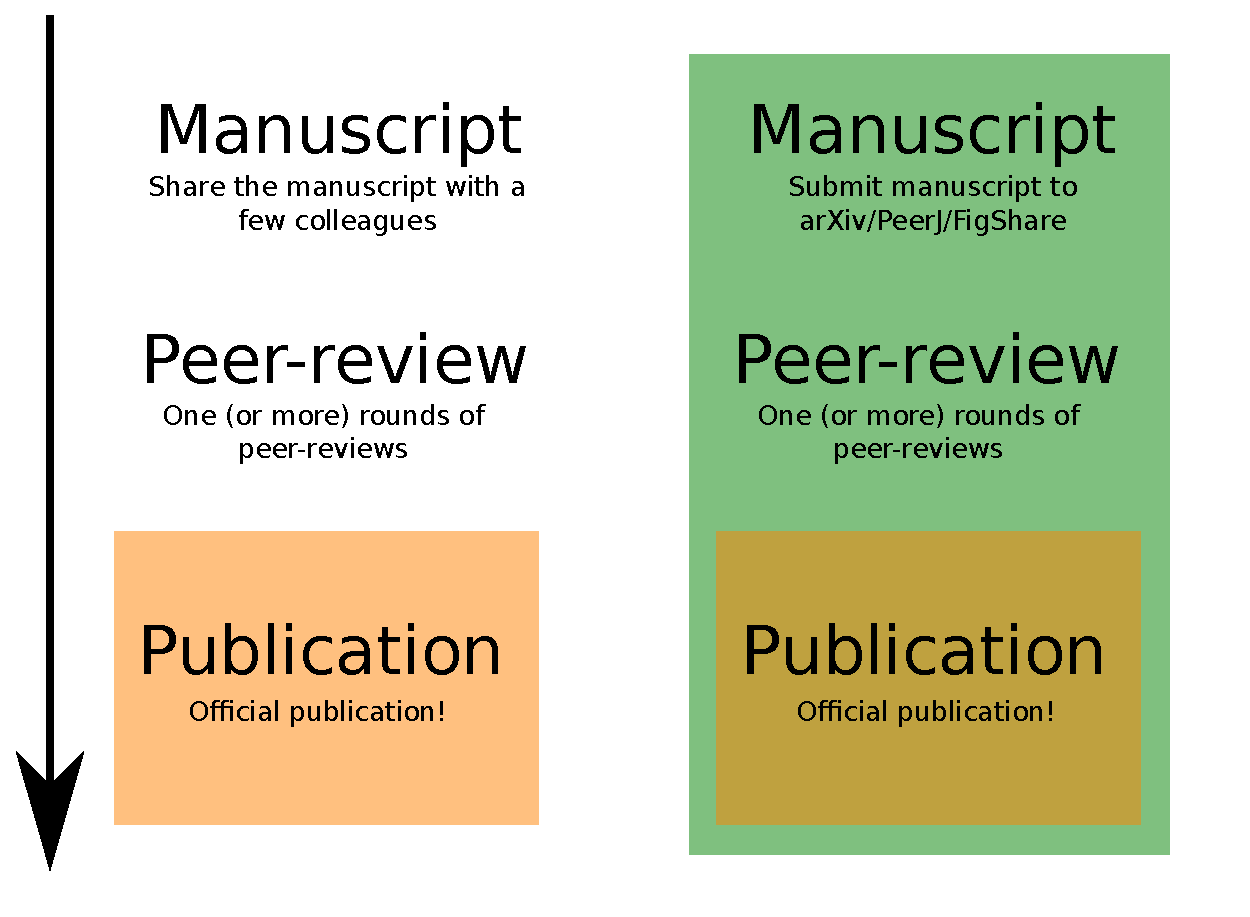
\includegraphics[width=0.50\textwidth]{map.pdf}
\caption { It can take several months, and even a few years, before a submitted
paper is officially published and citable.  The average time to publication
varies greatly between journals and can be as low as 104 days (Evolution for
2011) to 213 (PLOS One in 2010).  Meanwhile, few people are aware of the
research that has been done since, typically, only close colleagues are given
access to the preprints. With public preprint servers, the science is
immediately available and can be openly discussed, analyzed, and integrated into
current research. It benefits both science and publishers. Both want the papers
to be well-known and cited, and public preprints make it possible to integrate
research even before publication, greatly improving immediacy.  }
\label{fig:map} \end{figure}

Finally, public preprint servers offer a fair way to establish intellectual
priority by making the work available as soon as it is complete. Some
manuscripts will spend much more time in the review process and/or in
production after acceptance, than others. This means that publication and
acceptance dates do not accurately characterize who came up with an idea
first. For this reason, mathematicians and physicists have embraced arXiv in
part to establish priority in a fair way \cite{gin11,cal12}. This can be
especially crucial to early-career scientists. The sometimes long delay before
publication is seldom compatible with the pressure to show an impressive
publication record when applying for a scholarship or a position. Increasing
the perceived value of pre-prints as close, or equal, to journal articles (a
point we discuss in the conclusion) will allow young researchers to put their
research outcome in the open, and build a reputation for themselves through
the diffusion of their work, without the fear that this work will not be
recognized by grant or job commitees.

%%% TP Oct 11 2012
%%% Important to appeal to the young folks, while at the same time calling for
%%% more recognition of preprints. Feel free to rephrase, but don't remove!

\section{Preprints in biological sciences}

In contrast to other disciplines, the field of biology has effectively no
%%% TP
%%% As good a place as any to define biology... PLoS Biology, for example,
%%% is mostly cell biol stuff. We are not a typical subset of biologists!
preprint culture, with the exception of small pockets of primarily highly
quantitative research (\emph{e.g.}, epidemiology, population genetics).
Submitting to preprint servers has become more common in the past few years,
and the quantitative biology section in arXiv is experiencing the fastest
growth in submissions \cite{cal12}. Yet, the number of biology papers
submitted to preprint servers still represents only a small fraction of the
total research produced in biology.

There are a number of reasons that biologists have not traditionally had a
culture of sharing preprints, many of which are based on common misconceptions
regarding the costs and benefits associated with the practice. For example, in contrast
to other fields there is a perception in biology that public preprints
make it easier to steal ideas. However, there is no evidence of this happening
in the numerous other fields that have adopted preprint servers, and since preprint
servers create a clear record of who had the idea first, and when, this
appears to be a largely unfounded concern. In other fields preprints serve the
opposite role, they allow straightforward establishment of precedence, letting
research lay claim to an idea thus preventing it from being "stolen".
%%% TP
%%% Most refs will ask for a ref at that point. At least, I will, but I'm so
%%% demanding that I'm part of why the review process sucks ;-)

Another major concern is that if a researcher posts a public preprint that
they will not be allowed to submit their paper to their journal of choice.
This is based on a certain interpretation of the Ingelfinger rule: scientists
should not publish the same manuscript twice \cite{alt96}. A preprint is
simply a document that allows ideas to spread and be discussed, it is not yet
formally validated by the peer-review system. This is why the majority of
publishers do not see arXiv and similar services as a violation of the
Ingelfinger rule, and it is not unseen to have a preprint reproduced almost
exactly in the published version.
%%% TP
%%% Steve Frank papers on ArXiV often end up almost unmodified in JEB
%%% I can dig up the two version so that we can cite them
Almost all of the major publishers in
biology are preprint-friendly, including: Nature Publishing Group, PLOS, BMC,
PNAS, Elsevier, and Springer \ref{table:policies}. The Ecological Society of
America and the Genetics Society of America recently changed their
policies to allow public preprints. In fact,
\emph{Nature} responded to the rumour that they refused manuscripts submitted to
arXiv by saying that ``\emph{Nature} never wishes to stand in the way of
communication between researchers. We seek rather to add value for authors and
the community at large in our peer review, selection and editing'' \cite{nat05}.
Still, a few journals adopt a ``by default'' hostile attitude towards preprints,
mostly due to the lack of clear policy of the publishers, or perhaps because a
preprint culture has not developed in biology and the practice is still
considered unusual. As an example, Wiley-Blackwell, which publishes some of the
leading journals in biology, has no official policy on the matter.

\begin{table*}
    \centering
    \begin{tabular}{|ll|}
    \hline
    Publisher                                   & Policy \\
    \hline
    Springer                            	& Accept \\
    BMC                                 	& Accept \\
    Elsevier                            	& Accept \\
    Nature Publishing Group             	& Accept \\
    Public Library of Science           	& Accept \\
    Genetics Society of America                 & Accept \\
    Royal Society                       	& Accept \\
    National Academy of Science (USA)           & Accept \\
    Ecological Society of America       	& Accept \\
    Oxford Journals                             & Accept \\
    Science                             	& Ambiguous \\
    Wiley-Blackwell                       	& No general policy \\
    British Ecological Society                  & No answer to our query \\
    \hline
    \end{tabular}
    \caption{Policies for important publishers in biology. Some publishers
tolerate preprints except for a few of their medical journals, e.g.: Journal
of the National Cancer Institute from Oxford and The Lancer from Elsevier.}
    \label{table:policies}
\end{table*}

\section{Current offerings}

We briefly discuss the main options to submit preprints to open servers:
arXiv.org, figshare, and the upcoming PeerJ and F1000Research.

\subsection{arXiv}

arXiv (\url{http://arxiv.org/}) is the most widely-used preprint server today,
and its use is almost universal in some branches of mathematics and physics.
arXiv provides a reliable citation system for all eprints and is especially
popular in high-energy physics. Physicist Paul Ginsparg created arXiv in 1991
for theoretical high-energy physicists to communicate preprints via email and
ftp, and soon thereafter adopted the newly created world-wide
web\cite{jackson2002preprints}.  arXiv now receives over 7 000 submissions per
month (\url{http://arxiv.org/show_monthly_submissions}) and divides its
submissions into subcategories of physics, mathematics, computer science,
quantitative biology, finance and statistics.  The quantitative biology category
includes subcategories for Populations and Evolution, Quantitative Methods and
other categories that may be of interest to biologists.

One aspect of arXiv that differs from other options is that it has a moderation
system, which requires that papers must be categorized by an endorser.
At least one author of a paper must be an endorser that has previously submitted
a paper or has received permission to submit to a particular category. arXiv is now
administered by the Cornell University Libraries, with funding coming from
voluntary pledges by academic institutions along with matching funds from the
Simons Foundation \cite{arxiv_future}. This approach to financing is one of
the numerous measures that arXiv takes to ensure that the repository will remain
permanently available and submissions will be readable.

\subsection{figshare}

figshare (\href{http://figshare.com}{http://figshare.com}) is an open server
that allows scientists to submit any research output: manuscript, figures,
datasets, videos, theses, presentations, and so on. There are no rules to limit
what constitutes a research output and, unlike arXiv, there is no endorser
system. All figshare content has a unique digital object identifier (DOI) like
any journal article, thus offering a permanent and stable link to the content.
A flexible tag system is used to classify each item. Comments can be made on all
content allowing for centralized discussion related to the material.

One of the advantages of figshare over arXiv for biologists is that is it not
limited to quantitative sciences. arXiv.org has sections on quantitative biology
but might not be appropriate for non-quantitative work. With its flexible
approach to preprints, figshare offers an alternative to arXiv for empirical
biologists. Furthermore, by allowing all types of content, figshare also
provides an archive for early results (e.g.: figures, lab presentations).

\subsection{PeerJ}

PeerJ (\href{https://peerj.com/}{https://peerj.com/}) is a new Open Access
publisher that combines both a preprint server, and a peer reviewed journal.  It
is focused on the biological and medical sciences, which may help overcome the
perception that preprints do not have a place in biology. Like figshare this is
an advantage relative to arXiv for biologists doing non-quantitative work.  Also
like figshare, PeerJ allows commenting on posted preprints, improving the
potential for pre-publication dialog. In addition, preprints can be made private
if the authors choose, and shared only with selected colleagues. While this
reduces many of the benefits of preprints described above, it may allow some
researchers who would not otherwise post preprints to begin to explore the
possibility in a manner appropriate to their current circumstances.

In contrast to other preprint servers users cannot post unlimited public
preprints for free. One preprint per year can be posted for free, with a onetime
(\emph{i.e.} lifetime) fee of 99 dollars required to allow an author to post unlimited
public preprints. The preprint server is not tied to the journal, so preprints
can be posted regardless of where they will eventually be submitted for
publication.

\subsection{F1000Research}

F1000Research is not a public preprint server like the previous three servers.
Whereas arXiv, figshare, and PeerJ offer an option to submit a manuscript
without having it reviewed, papers submitted to F1000Research will eventually
be reviewed. Thus, F1000Research offers a hybrid model with publicly available
manuscripts at time of submission and standard peer-reviews that occur as part
of the submission process. Manuscripts are considered ``accepted'' and will
only be indexed after two positive referee responses. F1000Research works
closely with data providers to integrate raw data to the paper. For instance,
upon submitting a paper, authors are asked to upload their data, which are then
integrated in \emph{e.g.} figshare widgets, the DOI of which are given in the
paper when the data are first mentioned.  By integrating data to the paper,
F1000Research is working to make science more reproducible and open.

\subsection{GitHub}

This manuscript was developed entirely as an open project on GitHub. GitHub is
one of several hosting services for collaborative development using the Git
version control system (VCS).  Git is a decentralized revision control system
created by Linus Torvalds and is used primarily to develop software, including
the Linux kernel. Git provides powerful features that allow numerous
contributers to work asynchronously on the same project, often in parallel
branches, all of which can be effortlessly merged and version controlled.  While
Git is created primarily for software development, where the use of version
control systems is standard \cite{aru12}, it is ideal for academic research
since it provides a way to collaborate on every step of the manuscript
development process, from data manipulation and analysis to writing and
revision. For example, during the development of this manuscript, each author
would clone the project (\emph{i.e.} make a personal copy), modify it, and then
merge their changes into a master branch. This takes the preprint process to an
entirely new level, where the entire writing process is open from the beginning.

\section{Conclusion}

The ongoing discussions on the publication process, peer-reviewing and
alternative publication models are all symptoms of the current uneasiness of
scientists with the ever growing obsession with bibliographic metrics such as
the impact factor \cite{Fisher2012}. There is pressure on researchers to orient
their publication strategy in order to maximize their number of publications and
total citations. A well-known consequence is to submit manuscripts first to the
most prestigious journals, and then resubmit to ``lower level'' journals as they
are rejected. The numerous negative impacts of such behavior have been discussed
in depth \cite{hoc09} and include a long delay between the time a manuscript is
finished to its publication.  They all contribute somehow in a general slowing
down of scientific progress.  Research activities and the publication process
are drifting away from their fundamental object, namely the diffusion of novel
scientific discoveries. 

Developing a preprint culture in biology will not solve all problems with the
current publication process. It might however reduce significantly its negative
consequences. Preprint servers speed up publication and make no judgement on
pertinence and originality. Paradoxically, because peer-reviewing is conducted
\emph{after} this step in the process of scientific communication, it might
bring it closer to its fundamental objective. The role of peer-reviewing is to
judge the scientific quality of a study. The peer review process is the first
barrier against the fraudulent and poor quality science susceptible to impede
scientific progress. However, it is now dominated by subjective evaluations,
where trendy contributions are promoted to increase impact factors. Preprints
are by definition not evaluated, neither for their quality nor their pertinence.
Technically, the difference between a preprint and a traditional publication
should be that the latter as the approval stamp by pairs on its quality. The
relevance of a study, its contribution to science, should only be judged
post-publication by many more readers than the typical two-four anonymous
reviewers. With a such a shift in the diffusion strategy, the role of
traditional journals and their editors would be to showcase scientific
discoveries for specialized readership. Such a process should improve even
further their diffusion, not impede it. 

One of drawback of making publication easier is the proliferation of studies of
uneven quality. A trade-off between the intensity of the peer-review filtering
and the benefits to science has been hypothesized \cite{Aarssen2012}.  With
increasingly stringent peer reviewing, the quality of published papers and
easiness of finding discoveries might increase, at the cost of censorship, an
increased load on authors and reviewers, and greater delays for publication.
Preprints are simply bypassing this model for what we believe is the progress of
science: they speed up the dissemination of scientific discoveries, impede
censorship and put on reader's shoulders the responsibility to judge originality
and pertinence.

\section{Funding}

PDP is supported by an Alexander Graham Bell scholarship from the National
Sciences and Engineering Council of Canada. EPW is supported by a CAREER Award
from the National Science Foundation (DEB-0953694). JJA is supported by NSF
DEB-0614166 and NSF DEB-0919018.  TP is supported by a FQRNT-MELS post-doctoral
scholarship and 25 cents found by a coffee machine.  KR is supported by NSF
DEB-1021553. DG is funded by a Discovery Grand from the National Sciences and
Engineering Council of Canada and by the Canada Research Chair program.

\section{Acknowledgements}

We thank Carl Boettiger and Mark Hahnel for helpful comments on an earlier
version of this manuscript.

\newpage
\bibliography{refs}

\end{document}

